\section{Introduzione}

\subsection{PadovaCard ora}
PadovaCard è un pacchetto ideato per chi desidera visitare la città. 
I punti di forza sono:
\begin{itemize}
\item Utilizzo gratuito dei mezzi di trasporto pubblici comunali;
\item Parcheggio gratuito in alcune zone;
\item Noleggio di veicoli, biciclette, segway a prezzo scontato;
\item Accesso gratuito alle strutture convenzionate.
\end{itemize}
\`E acquistabile con validità di 48 e 72 ore, contate dal momento in cui la PadovaCard viene ritirata allo sportello informazioni assistenza turistica (\glossario{IAT}).
La carta si presenta come in figura \ref{immaginePadovaCard}, e non presenta nessun tipo di circuito, banda magnetica o codice stampato. 
Proprio per questo motivo, nonostante sia una tessera personale e non cedibile, non c'è modo di verificare chi ne è l'intestatario.\\

\begin{figure}[H]
\centering
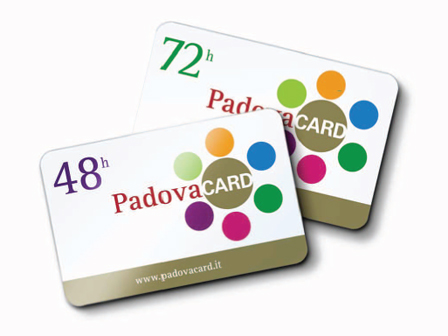
\includegraphics[width=0.6\textwidth]{images/padovacard.jpg}
\caption{Veste grafica dell'attuale PadovaCard}\label{immaginePadovaCard}
\end{figure}

Per acquistare una PadovaCard l'\glossario{utente} può recarsi ad uno degli sportelli IAT che si trovano sul territorio della città di Padova o in uno dei punti vendita autorizzati (hotel, tabaccherie, etc.).\\

\label{cappella}
La \cappella è uno tra i luoghi d'interesse più visitati, ed è convenzionato con PadovaCard. La visita alla cappella presenta un ingresso contingentato, ovvero il numero di visitatori per ogni visita è fissato, e per questo è necessario prenotare la propria visita, definendo data e fascia oraria. Non è possibile visitare la \cappella senza prenotazione. \\

Questo vincolo fa si che chiunque acquisti una PadovaCard con l'intenzione di visitare la \cappella è obbligato a prenotarne la visita. Questo è possibile farlo se si acquista la PadovaCard in un punto vendita autorizzato, oppure attraverso la piattaforma \vivaticket.
\`E inoltre attivo un call center che permette agli utenti di acquistare una PadovaCard collegata ad un ingresso in \cappella.
In questi ultimi due casi la PadovaCard verrà poi ritirata presso un punto vendita o direttamente alla \cappella.\\

I principali problemi di funzionamento dell'attuale PadovaCard sono:
\begin{itemize}
\item La PadovaCard non è nominativa;
\item Il sistema non è informatizzato e non prevede alcun tipo di tracciamento;
\item L'utente è obbligato in tutti i casi a passare da uno IAT per il ritiro della PadovaCard;
\item La piattaforma di vendita è frammentata e non comunica pienamente le offerte della PadovaCard;
\item Il sistema di vendita è frammentato tra OSS e \tlite.
\end{itemize}

La nuova PadovaCard si pone l'obbiettivo di risolvere questi problemi.



\subsection{OSS}\label{oss}
\subsubsection{Overview}
\glossario{OSS} è una piattaforma sviluppata da \net per la gestione del call center e degli sportelli \glossario{IAT} e dei relativi operatori.
Gli operatori si autenticano su questo software per gestire la vendita dell'attuale PadovaCard\footnote{Sia OSS che \tlite possono vendere la PadovaCard, salvando i dati relativi alla vendita in due diverse basi di dati. SI tratta di un problema dell'attuale sistema.} e di ogni altra merce in vendita agli sportelli \glossario{IAT}. 
OSS permette agli operatori di visualizzare il rendiconto delle vendite e al personale operatvio di compiere interrogazioni sulla base di dati.

\subsubsection{Dettagli tecnici}
Il software è scritto in \glossario{Cake Php} e si basa sull'architettura \glossario{MVC}. Come previsto da MVC sono presenti dei model, uno per ogni tabella del database, tali model si occupano di comunicare col database e di manipolare e verificare i dati che vengono estratti ed inseriti.
Per ogni model è presente un controller, che fornisce la logica al sistema attraverso vari metodi. Ad ogni controller sono collegate più view, ovvero le interfaccie utente. Una view è una pagina con cui l'utente interagisce e ogni view deve essere associata ad un controller di cui chiamerà i metodi.\\

Il database su cui si basa il sistema è un database \glossario{MySql}.

\subsection{\tlite}
\tlite è il software sviluppato da \charta che si trova dietro la piattaforma \vivaticket, e che gli operatori utilizzano per gestire la vendita delle PadovaCard\footnote{Vedi nota 1.} con annessa prenotazione alla \cappella.
Non trattandosi di un software sviluppato da \net si è dovuto adattare i requisiti ai limiti imposti da tale software.
Il limite principale è la mancanza di comunicazione tra \tlite e il software sviluppato causato da una mancanza di \glossario{API} pubbliche di \tlite.\\

Si sono comunque rivelate necessarie alcune modifiche minori al software e per questo è stato svolto un incontro tra gli sviluppaotri di \tlite e quelli di \net.
Ai fini di questo documento non è necessario conoscere il funzionamento di \tlite nel suo insieme, mentre i punti d'interesse per la progettazione del nuovo sistema per PadovaCard saranno presentati nella sezione \ref{progettazione}.

\subsection{Lavoro svolto}
Il focus dello stage è stato sui seguenti punti:
\begin{itemize}
\item Analizzare i requisiti del sistema PadovaCard, il risultato è visibile alla Sezione \ref{analisideirequisiti};
\end{itemize}

\subsubsection{Analisi dei requisiti}
Di seguito viene descritto l'approccio seguito per generare una dettagliata analisi dei requisiti, il cui risultato è presentato nella Sezione \ref{analisideirequisiti}.
L'azienda \net ha fornito al tirocinante un documento in cui vengono descritti gli obbiettivi e le criticità del nuovo sistema per la Padovacard. Dallo studio di tale documento il tirocinante ha potuto definire il piano di lavoro dello stage.\\

L'analisi degli obbiettivi e del funzionamento del sistema ad alto livello è stato poi discusso in diverse riunioni tra i membri del team di sviluppo, ponendo un focus particolare sulle difficoltà inerenti alla \cappella, esposte nella Sezione \ref{cappella}.\\

Da queste riunioni il tirocinante ha estratto i dettagli funzionali dell’applicazione.
Per esprimere in modo chiaro i requisiti individuati si è ricorso al formalismo UML - Casi d'uso, anch'essi visionabili alla Sezione \ref{analisideirequisiti}.\\

L'individuazione dei requisiti è stata fatta corretamente già alla prima iterazione, mentre i casi d'uso e la loro descrizione dettagliata sono stati modificati più volte, al fine di eliminare ogni possibile ambiguità.
\subsection{Risultati a fine stage}